\chapter{Explorarea setului de date}

\section{Descriere}

Acest set de date conţine informaţii despre 284,807 de tranzacţii dintre care 
492 sunt \textbf{frauduloase}. Conţine doar variabile numerice.

Din motive de confidenţialitate, dimensiunea trăsăturilor originale a fost 
redusă folosind \textbf{Analiza Componentelor Principale} (PCA) la 28 de trăsături denumite 
"V1-V28" şi încă 2 trăsături ce nu au fost transformate, anume suma de bani
a tranzacţiei şi timpul relativ, începând de la 0, când aceasta a fost făcută. 
De asemenea, pentru fiecare tranzacţie avem eticheta 0 sau 1, daca este normală 
sau, respectiv, frauduloasă.

\section{Matricea de corelaţie}

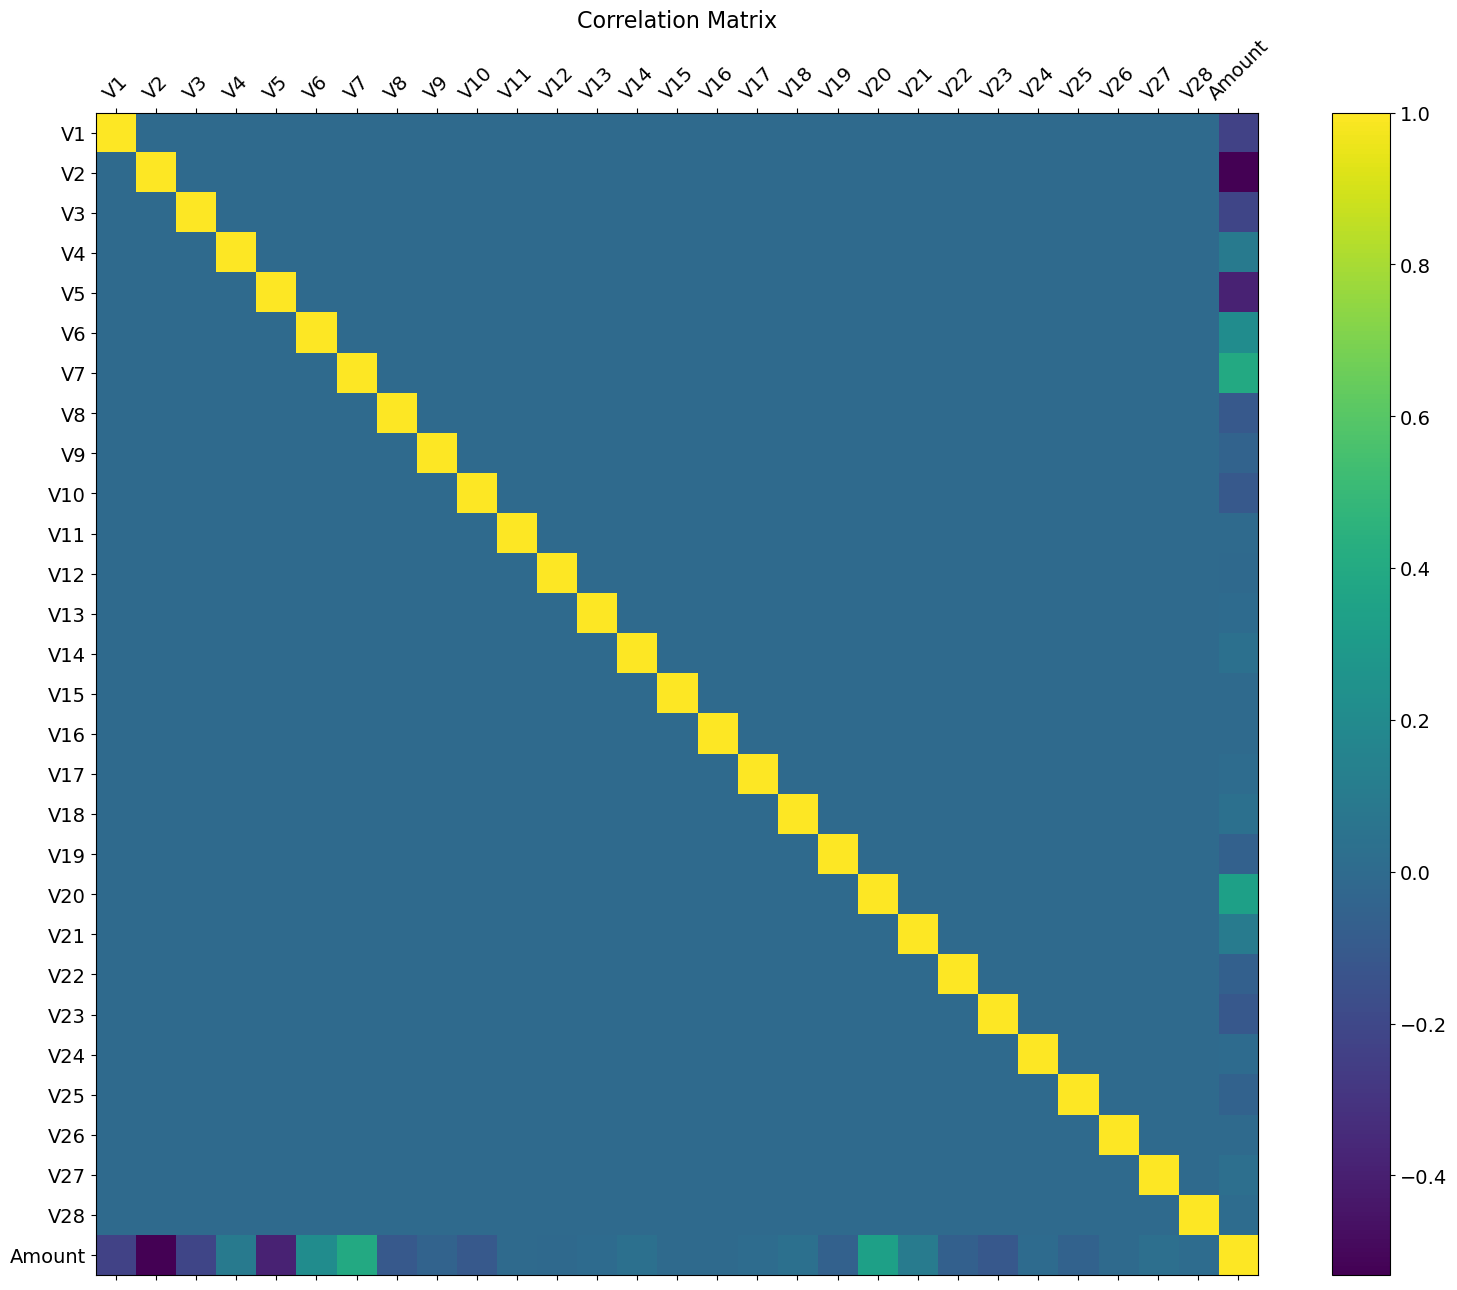
\includegraphics[width=\linewidth]{correlation-matrix.png}

Se observă lipsa corelaţiei între variabilele anonime. Este de aşteptat, totuşi, 
având în vedere că variabilele au fost obţinute prin PCA, care din definiţie generează 
componente \textbf{necorelate liniar}.

Singura corelaţie apare între variabila "Amount" şi restul variabilelor. Corelaţiile
cu o magnitudine semnificativă apar între amount şi V6, V7, V20, cu valoare pozitivă, 
şi între amount şi V1, V2, V5, cu valoare negativă.

\section{Preprocesarea datelor}

\subsection{Eliminăm trăsăturile inutile}

În viaţa reală, data şi ora tranzacţiei ne pot ajuta să depistăm un comportament 
ciudat. Totuşi, aceste informaţii sunt relevante numai atunci când am monitorizat
pe o perioada de măcar câteva zile activitatea din contul/cardul respectiv pentru a 
stabili ce reprezintă un comportament "normal".

În cazul nostru, nu avem la dispoziţie nici măcar data şi ora exactă. Prin urmare, vom
elimina timpul din fiecare observaţie.

De asemenea, eliminăm etichetele. Acestea sunt utile numai la testare pentru a analiza 
performanţa şi la alegerea setului de antrenare. Metodele utilizate în această lucrare
sunt exclusiv \textbf{nesupervizate}, deci nu avem nevoie de etichete la procesul de antrenare.

\subsection{Validarea încrucişată}

Împărţim setul de date în antrenare, validare şi testare cu proporţiile 75\%, 0.15\%
şi, respectiv, 0.10\%. De asemenea, ne asigurăm că 
\textbf{proporţiile de normal/anomalie} 
rămân aproximativ la fel în toate seturile.

Totuşi, pentru că algoritmii prezentaţi "învaţă" structura datelor normale şi avem 
la dispoziţie etichetele, vom elimina din \textbf{setul de antrenare}
toate punctele cu eticheta 
1 şi le vom muta în setul de validare.

\textbf{Setul de validare} va fi folosit pentru alegerea hiperparametrilor optimi, în timp ce 
\textbf{setul de testare} va fi folosit la final pentru a face o comparaţie imparţială 
a performanţei modelelor.

\subsection{Scalare}

Având în vedere că nu cunoaştem mai nimic despre trăsăturile punctelor, vom scala 
datele folosind metoda clasică de 
\textbf{a scădea media şi a împărţi la deviaţia standard}.
Media şi deviaţia standard sunt obţinute din setul de antrenare. Le folosim pe acestea 
să transformăm setul de validare, cât şi pe cel de testare.